% Here is a template so that we can have consistent formatting

\section{Path traversal exposes all content in media}

All content in the \url{/media} folder can be accessed and downloaded through URL manipulation.

\subparagraph{Investigation:}

This vulnerability was found through information leaking by typing in a faulty path name.
\begin{center}
    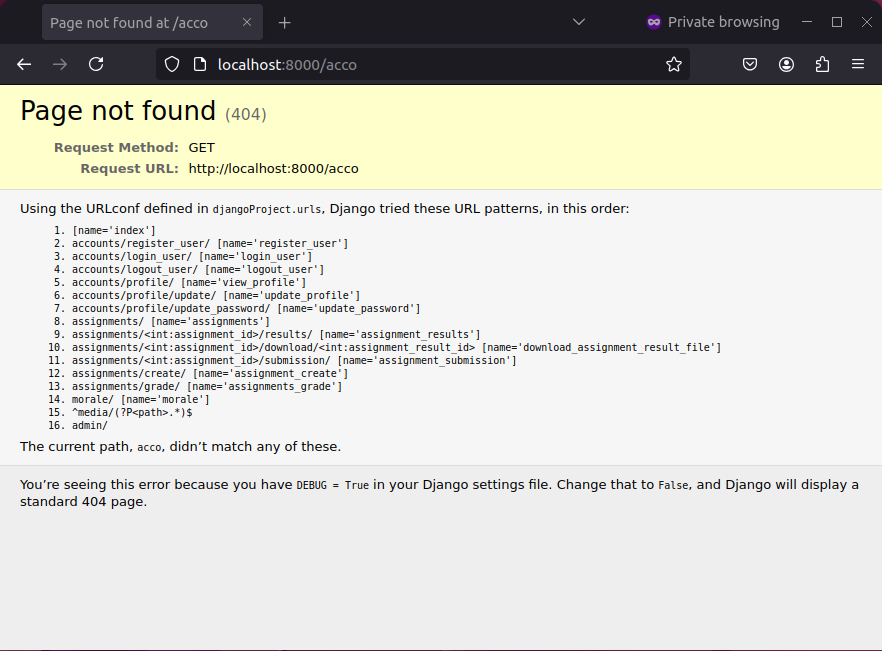
\includegraphics[width = \linewidth]{images/Michelle/debug.png}
\end{center}
This suggests that there exists a URL which utilises \url{/media} and a path associated with it, suggesting a relative path to a media folder in the code.

This is confirmed by checking the \url{/media} URL with any other filepath, e.g. \url{http://localhost:8000/media/sldkfls}:
\begin{center}
    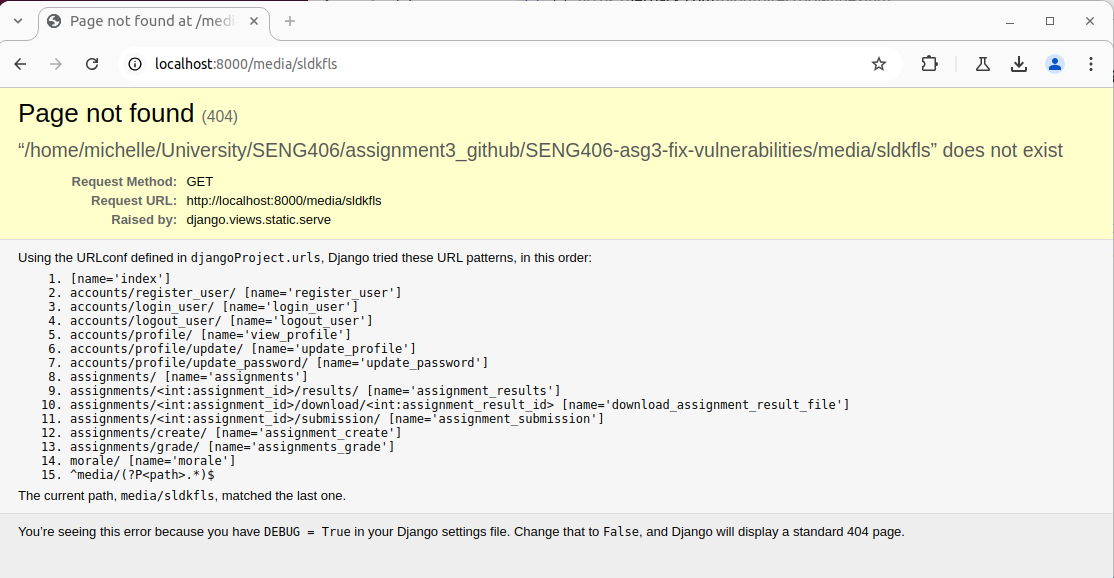
\includegraphics[width = \linewidth]{images/Michelle/pathleaking1.png}
\end{center}

This gives the error message listing the following URL: \url{/home/michelle/University/SENG406/assignment3_github/SENG406-asg3-fix-vulnerabilities/media/sldkfls} which leaks the directory structure of the file system.

\subparagraph{Exploitation:}

From here, exploiting this vulnerability can be done through brute force by trying common directory names. A successful directory find will result in the following error message:

\begin{center}
    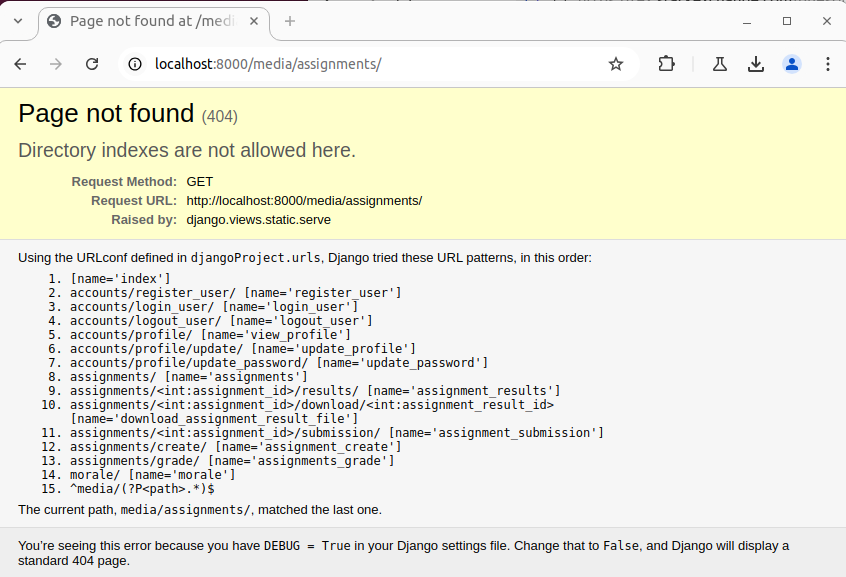
\includegraphics[width = \linewidth]{images/Michelle/directoryindex.png}
\end{center}

This gives information that "assignments" is a directory within media (stating "Directory indexes are not allowed here").

As the directory is named "assignments", one could assume that assignments could be stored here.

On submitting an empty assignment and then trying to download it, you get the following page:

\begin{center}
    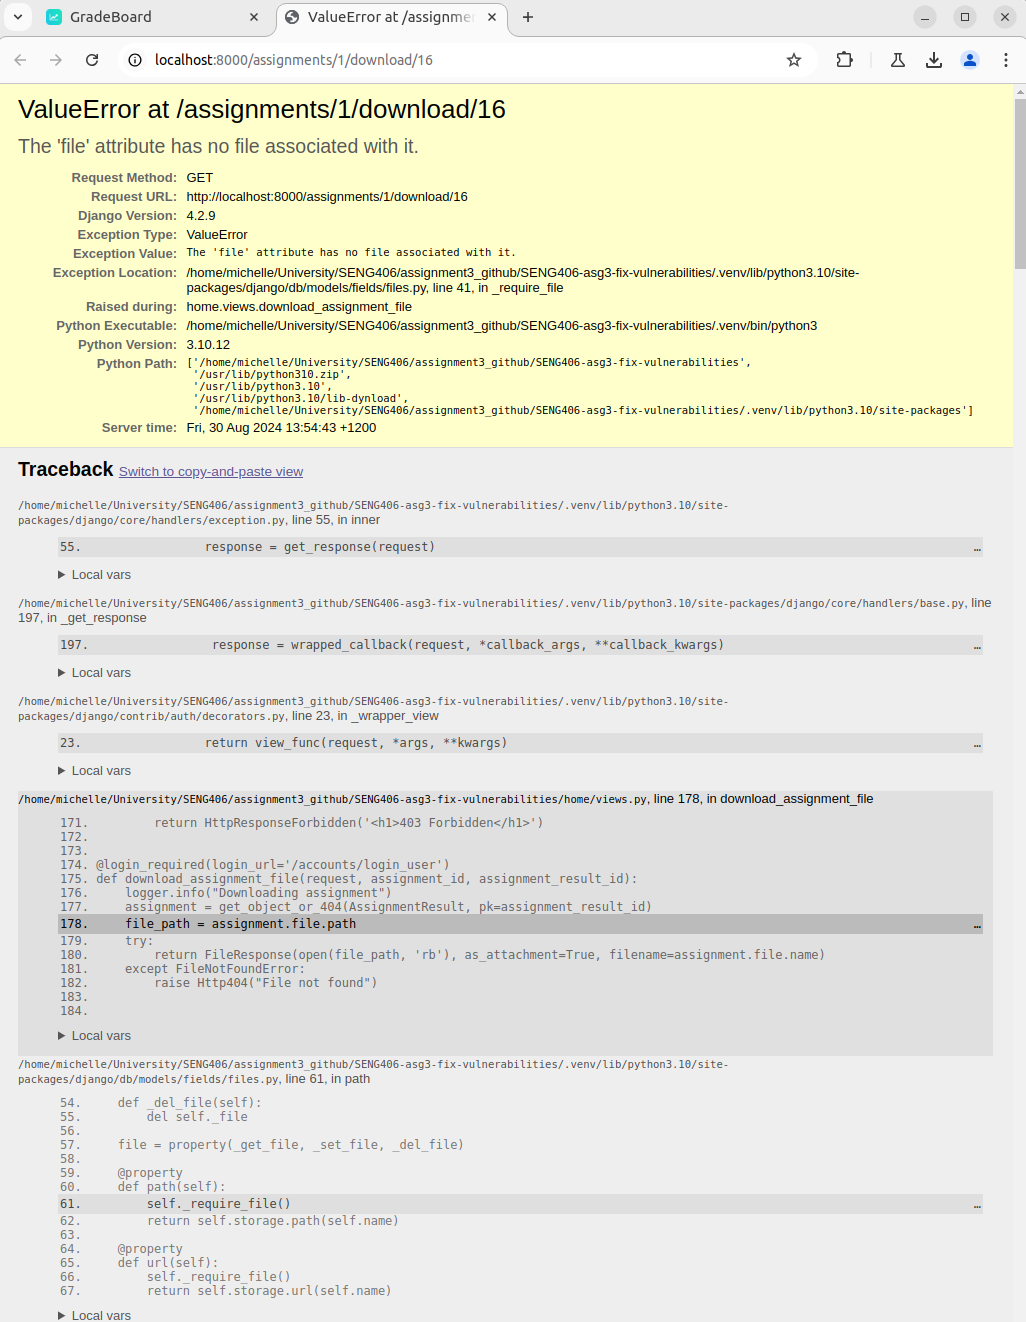
\includegraphics[width = \linewidth]{images/Michelle/filefinding.png}
\end{center}

This gives you information that the filepath is the name of the file uploaded.

From this information, you can then download anybody's assignment provided that you have the filename.

This will also occur for profile pictures (also stored in the exposed media directory).

You can also access the assignments results page without logging in (no authentication). From there, you can see the filepaths for each assignment submission.

\subparagraph{OWASP Top 10 Category:}

Broken Access Control

\subparagraph{Corrective Action:}

Delete line 24 in urls.py:

\begin{center}
    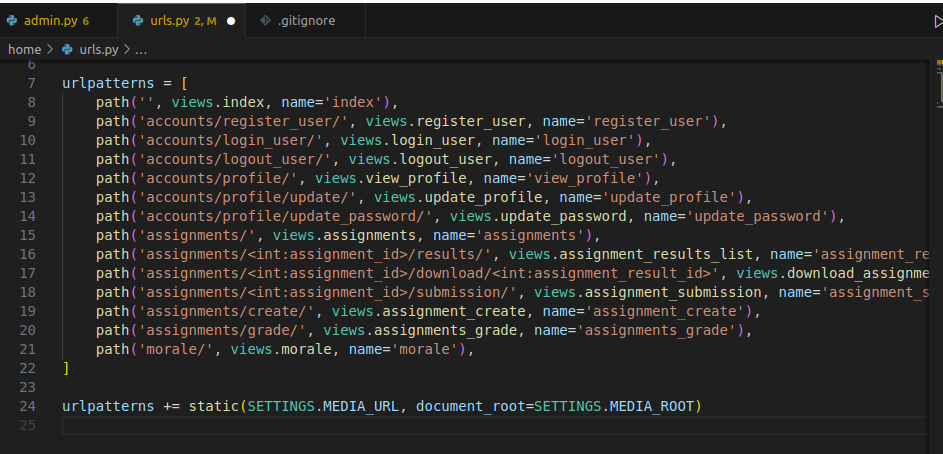
\includegraphics[width = \linewidth]{images/Michelle/media_fix.png}
\end{center}


\section{Accessible log files}

Log files are written and stored in the assignments directory. As assignments can be downloaded according to their filename, this log file can be accessed in multiple ways.

\subparagraph{Investigation:}

Upon uploading a file, it was noted that if you named a file \url{all.log}, then downloaded it, instead of downloading the expected uploaded file, a log file will be downloaded.

\begin{center}
    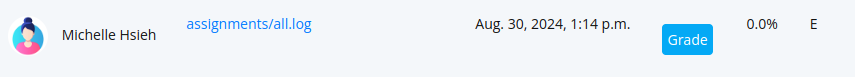
\includegraphics[width = \linewidth]{images/Michelle/logdownload.png}
\end{center}

\begin{center}
    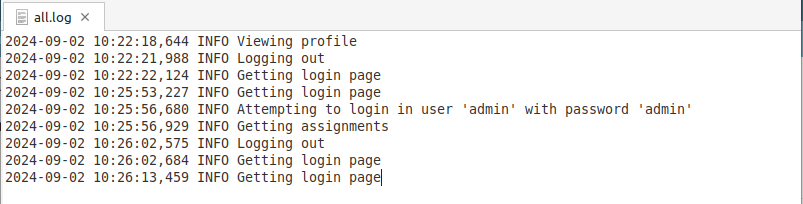
\includegraphics[width = \linewidth]{images/Michelle/logfile.png}
\end{center}

This can occur throughout the standard view and also in the admin view:

\begin{center}
    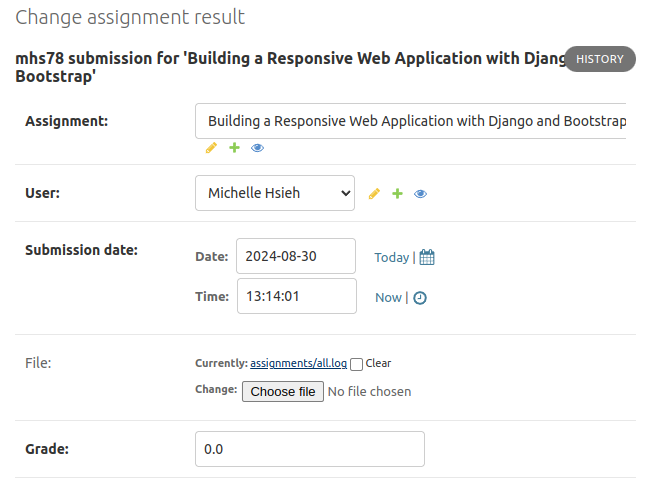
\includegraphics[width = \linewidth]{images/Michelle/logdownloadalt.png}
\end{center}

The log files should not be exposed to web-accessible locations, therefore should not be stored alongside assignments.

\subparagraph{Exploitation:}

This can be exploited as the log file contains some sensitive information, such as username and passwords, which can be used to maliciously log into other people's accounts.

\begin{center}
    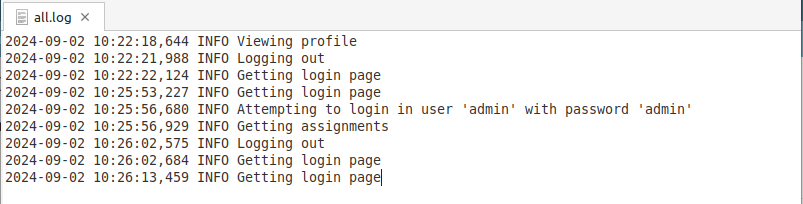
\includegraphics[width = \linewidth]{images/Michelle/logfile.png}
\end{center}

\subparagraph{OWASP Top 10 Category:}

Insecure Design

\subparagraph{Corrective Action:}

Following OWASP logging guidelines (\url{https://cheatsheetseries.owasp.org/cheatsheets/Logging_Cheat_Sheet.html}), the following was implemented: 

A separate directory was created labelled: \url{logs}. This ensures that the logs are not exposed in web-accessible locations and is in a separate partition to other application files and user generated content.

Line 155 in settings.py was rewritten so the handler write the log into the appropriate folder.

\begin{center}
    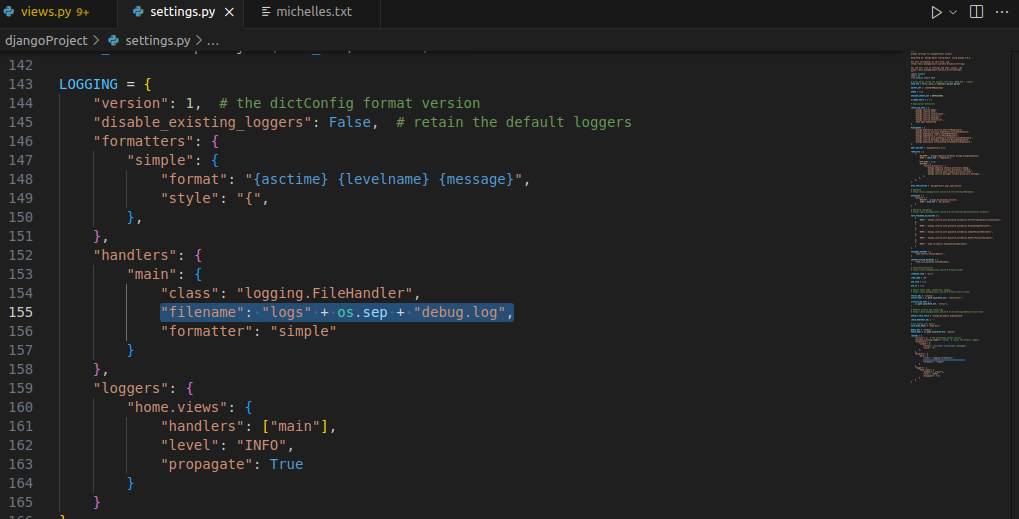
\includegraphics[width = \linewidth]{images/Michelle/logfix.png}
\end{center}

The old log file is removed.

\section{Assignment upload filename conflicts}

When uploading a file with a pre-existing filename, the new file is not uploaded, and attempting to download the new file leads to downloading the old file.

\subparagraph{Investigation:}

This was discovered by uploading an assignment with a particular name, say michelles.txt, with the following content:

\begin{center}
    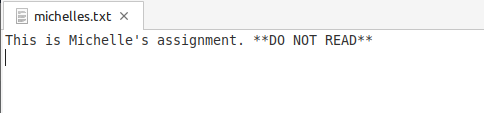
\includegraphics[width = \linewidth]{images/Michelle/michellestxt.png}
\end{center}

This was uploaded through the Local Weather App assignment.

\begin{center}
    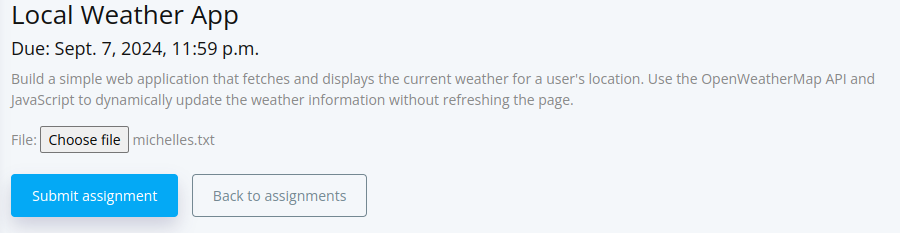
\includegraphics[width = \linewidth]{images/Michelle/submitone.png}
\end{center}

This was then downloaded, and the content was changed and then uploaded again. 

\begin{center}
    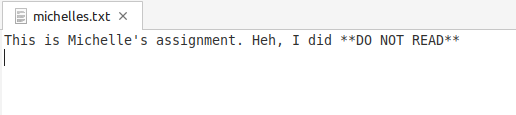
\includegraphics[width = \linewidth]{images/Michelle/michellestxt2.png}
\end{center}

Upon downloading the file again, no changes have occurred (the original file is still uploaded).

\subparagraph{Exploitation:}

This can be used to download someone else's assignment, provided that the filename is the same. 

To do this, another user (admin), uploaded a file titled: michelles.txt with no text.

Using the following Download button, that user was able to download the originally uploaded document by another user.

\begin{center}
    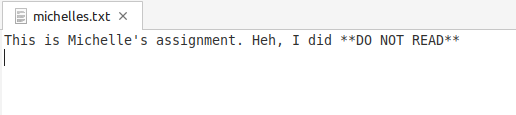
\includegraphics[width = \linewidth]{images/Michelle/michellestxt2.png}
\end{center}

This suggests that a) the original uploader's file is accessible to other users and b) the second uploader's file has not been uploaded.

Also, uploading no assignment is permitted, and downloading an absent assignment results in the following debug page being exposed:

\begin{center}
    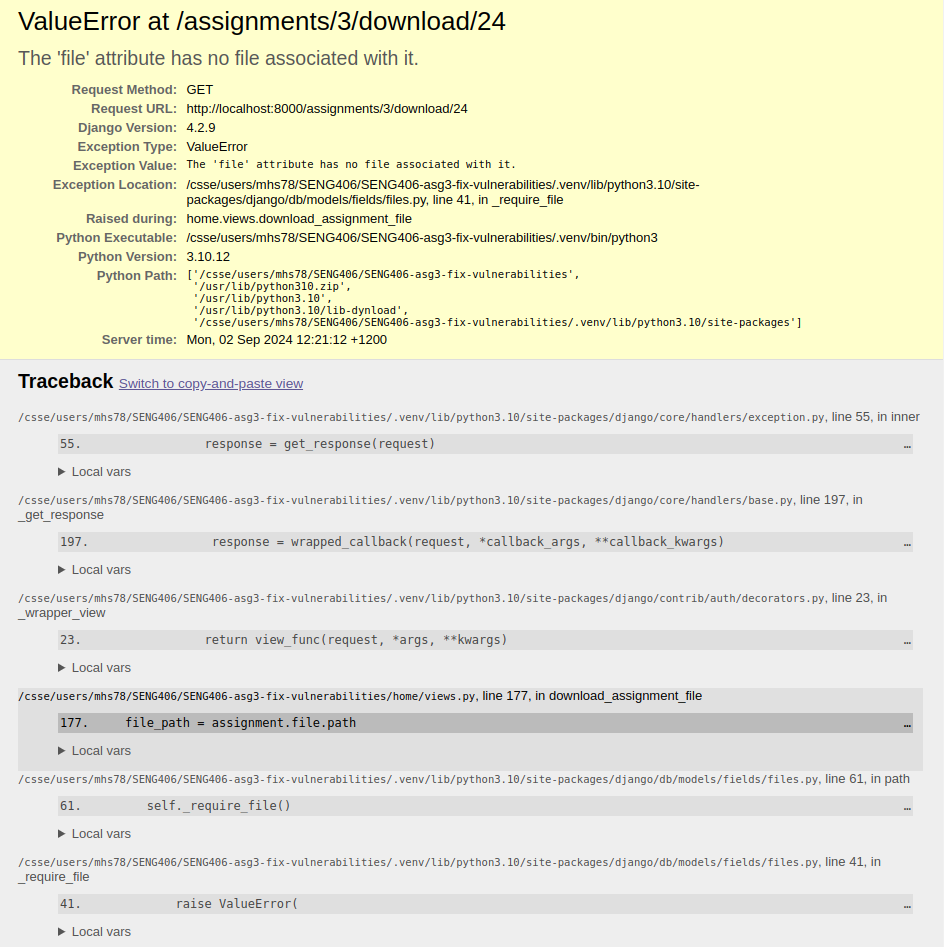
\includegraphics[width = \linewidth]{images/Michelle/noassignment.png}
\end{center}

\subparagraph{OWASP Top 10 Category:}

Broken Access Control

\subparagraph{Corrective Action:}

The following fix prevents assignments from being submitted incorrectly.

Changing line 30 on models.py:

\begin{center}
    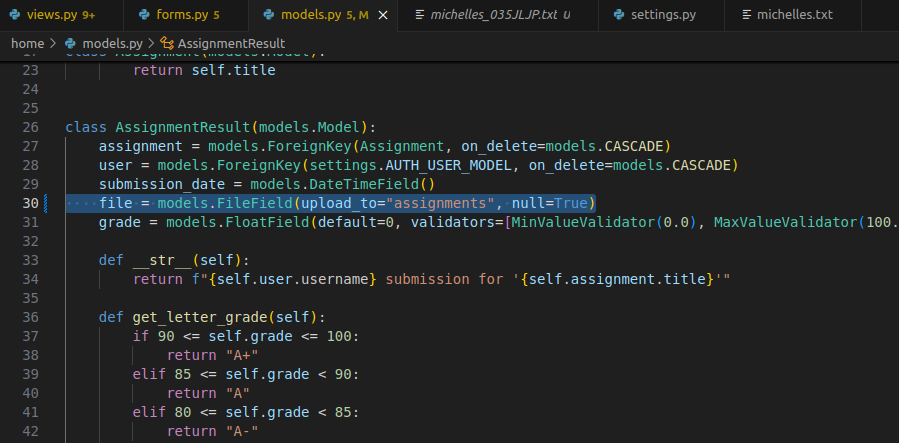
\includegraphics[width = \linewidth]{images/Michelle/fileuploadingchanges.png}
\end{center}

By removing the option blank=True, this stops the uploading of no files.

\begin{center}
    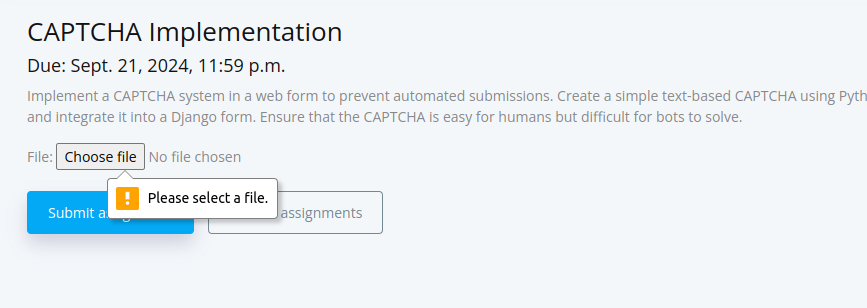
\includegraphics[width = \linewidth]{images/Michelle/needsfile.png}
\end{center}

By removing the ReuseExistingFileStorage class in models.py and the use of it in line 30, this allows Django's upload handler to deal with file uploading.

The use of ReuseExistingFileStorage returns a previously stored version of a file based on filename and prevents storing of multiple files of same filename. Removing this allows the saving of multiple files and prevents unintended file access as each filename is now associated with exactly one user.

\section{Download anyone's assignment}

It is possible to download anyone's assignment by intercepting and changing the GET request, or the HTML tag.

\subparagraph{Investigation:}

By inspecting the Download button on the assignments page, it appears that downloading assignments occur according to an ID.

\begin{center}
    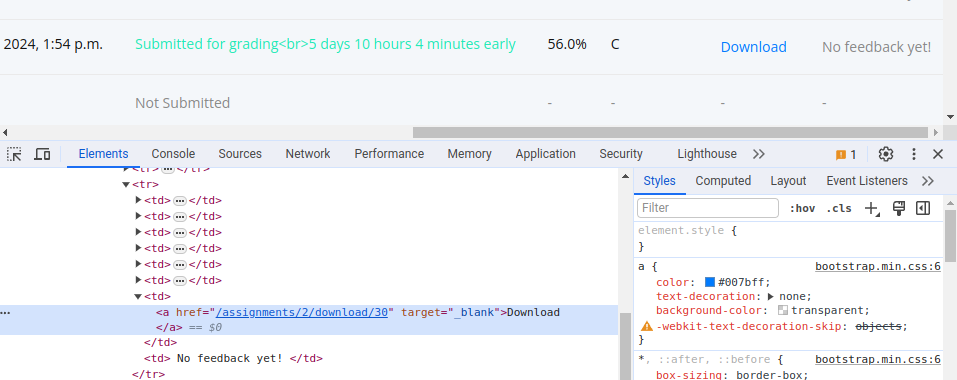
\includegraphics[width = \linewidth]{images/Michelle/downloadlink.png}
\end{center}

Using BurpSuite to intercept with the data, the following GET request is made:

\begin{center}
    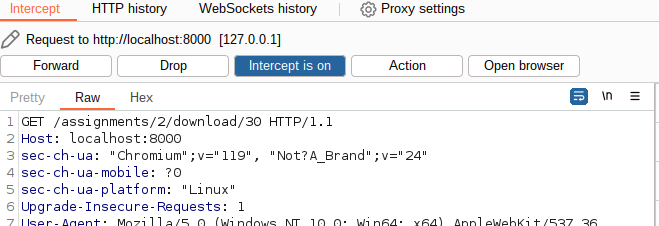
\includegraphics[width = \linewidth]{images/Michelle/interceptget.png}
\end{center}

Looking at the debug paths, it appears that two values are used to get data; the assignment number and the submission number:

\begin{center}
    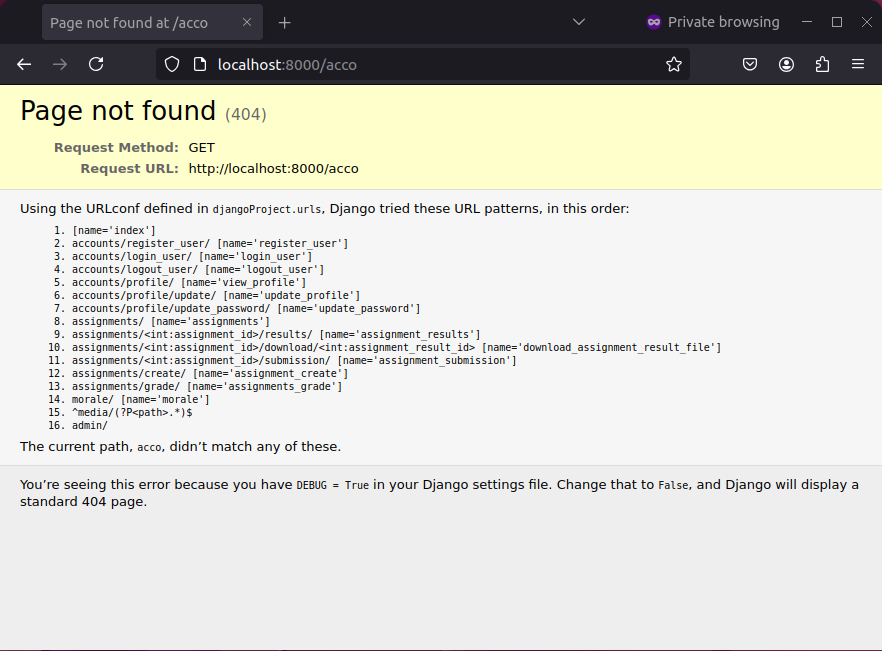
\includegraphics[width = \linewidth]{images/Michelle/debug.png}
\end{center}

This suggests a potential data leak if anyone could download anyone's assignment, provided they had two numbers which could be brute-forced.

Upon further investigation, varying the assignment number changes nothing, therefore only changing the assignment submission ID is necessary.

\subparagraph{Exploitation:}

By modifying either the HTML tag or the GET request, you can get any assignment. For instance:

\begin{center}
    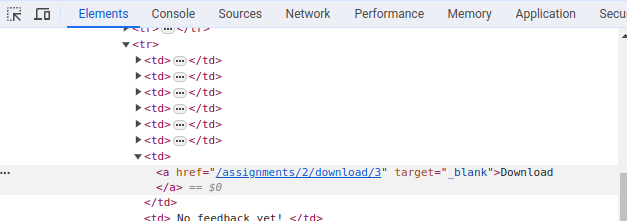
\includegraphics[width = \linewidth]{images/Michelle/altdownload.png}
\end{center}

Allows you to download Morgan's Captcha zip.

As the download is not verified, and the submission numbers are sequential, a user could submit one assignment, inspect the HTML of the download button to get the submission ID and successfully download everyone else's assignments (with prior submission IDs).

\subparagraph{OWASP Top 10 Category:}

Broken Access Control

\subparagraph{Corrective Action:}

In views.py, author checking is done by adding an if statement that checks if the user ID of the request matches that of the assignment and to give a 403 Forbidden response if they do not match.

Teacher status is also allowed access (else the teacher cannot download the assignment to mark).

\begin{center}
    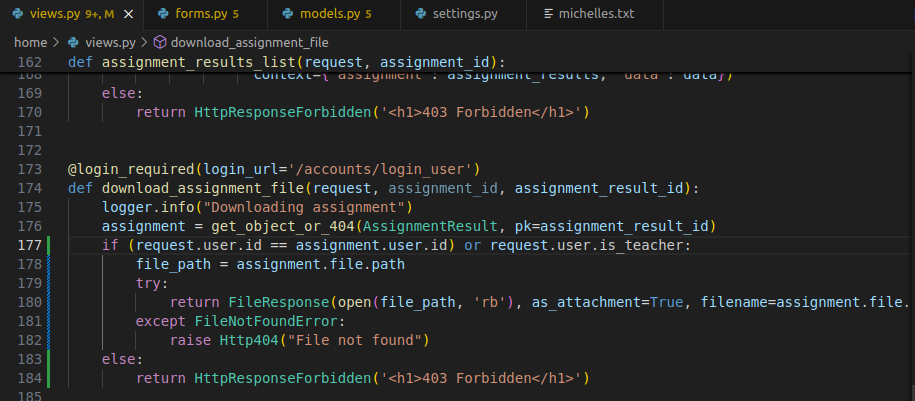
\includegraphics[width = \linewidth]{images/Michelle/assignmentgetfix.png}
\end{center}

\section{Morale API key exposed}

The API key for the morale-boosting cat images can be viewed.

\subparagraph{Investigation:}

By inspecting the image and the associated script tag, you can see the API key for the cat image API.

\begin{center}
    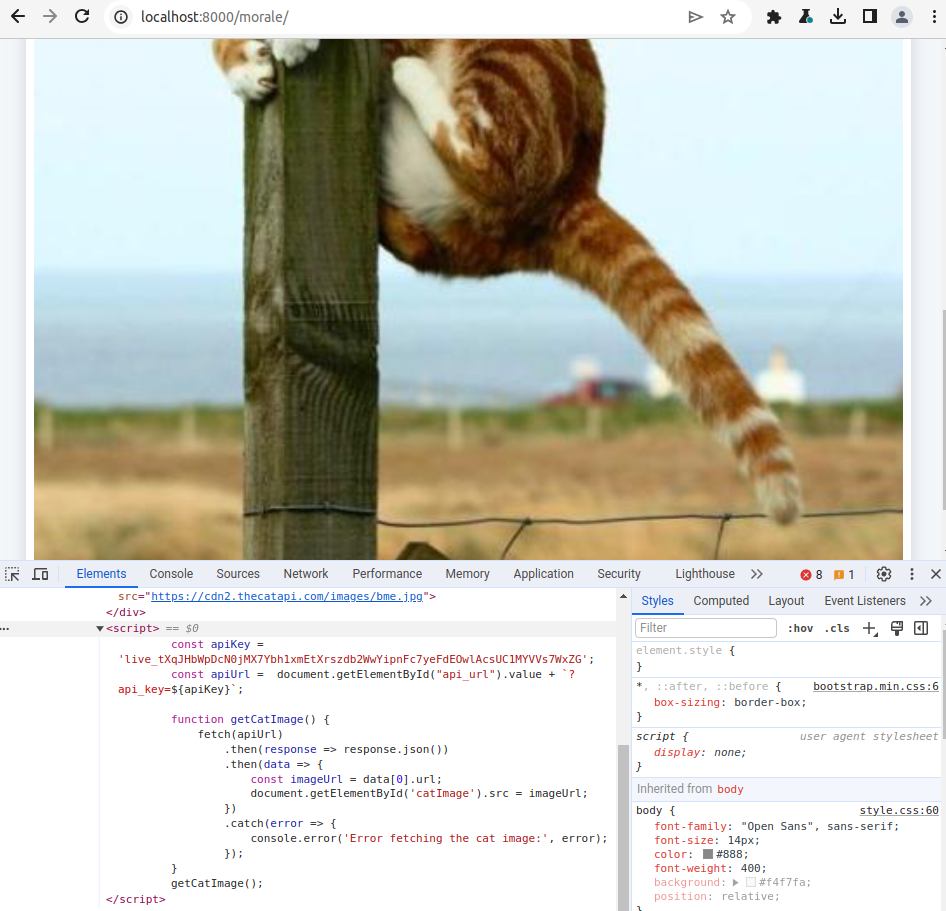
\includegraphics[width = \linewidth]{images/Michelle/morale.png}
\end{center}


\subparagraph{Exploitation:}

With this API key, you can then host your own cat image displaying server using someone else's API key.

This poses issues if there are limited requests per month (e.g. 10,000) or if there is payment required to use the API key.

\subparagraph{OWASP Top 10 Category:}

***To update: Broken Access Control?

\subparagraph{Corrective Action:}

The API key was taken out of the JavaScript in the morale.html file on lines 15-16.

The function using the Fetch API to get data directly from the cat API was changed to a POST request on the /morale endpoint (lines 19-27). JSON was used to send data regarding the API URL in the body of the POST request.

\begin{center}
    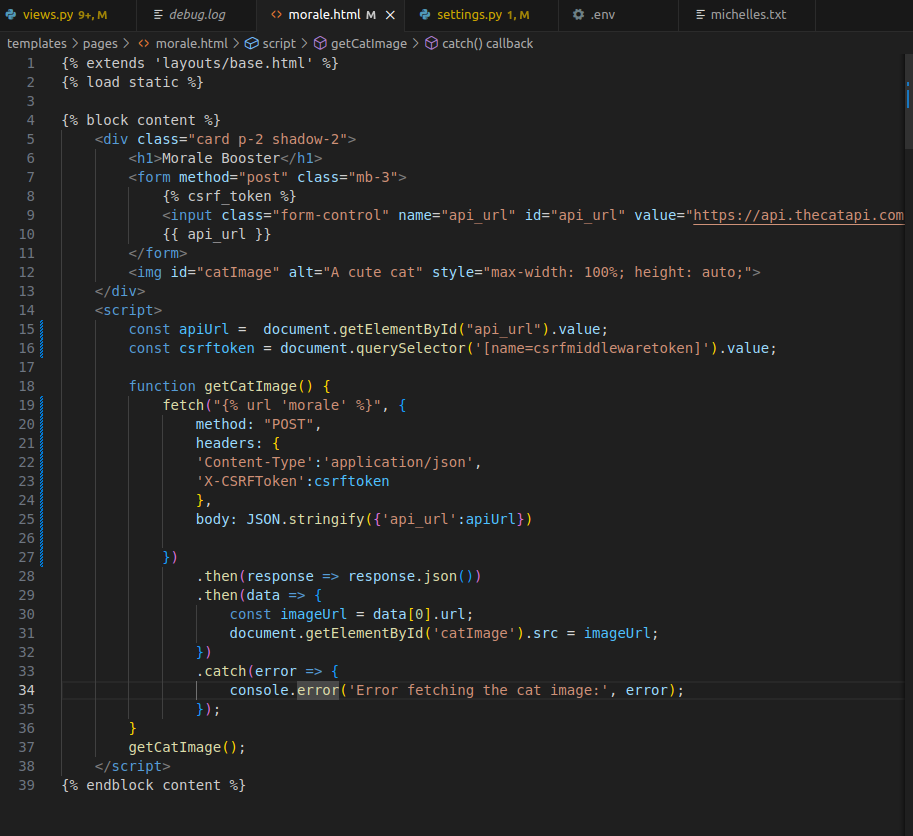
\includegraphics[width = \linewidth]{images/Michelle/jschanges.png}
\end{center}

A new .env file was created to store the API key. 

\begin{center}
    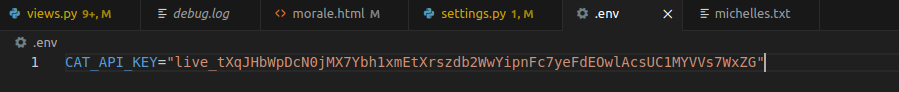
\includegraphics[width = \linewidth]{images/Michelle/envfile.png}
\end{center}

This was loaded using Python dotenv library in settings.py (lines 15-17, line 24) as the CAT\_API\_KEY:

\begin{center}
    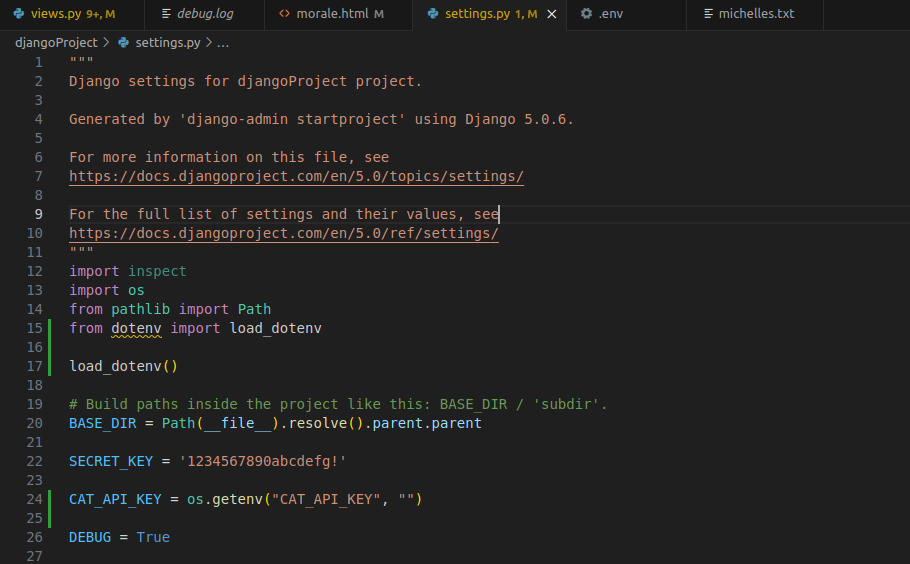
\includegraphics[width = \linewidth]{images/Michelle/APIkeyextraction.png}
\end{center}

On the /morale endpoint (in views.py), the JSON request data is decoded. On line 280, the cat API URL and the API key (loaded from the settings file) is used to request the data and return the cat content.

A testing of this fix shows the following:

\begin{center}
    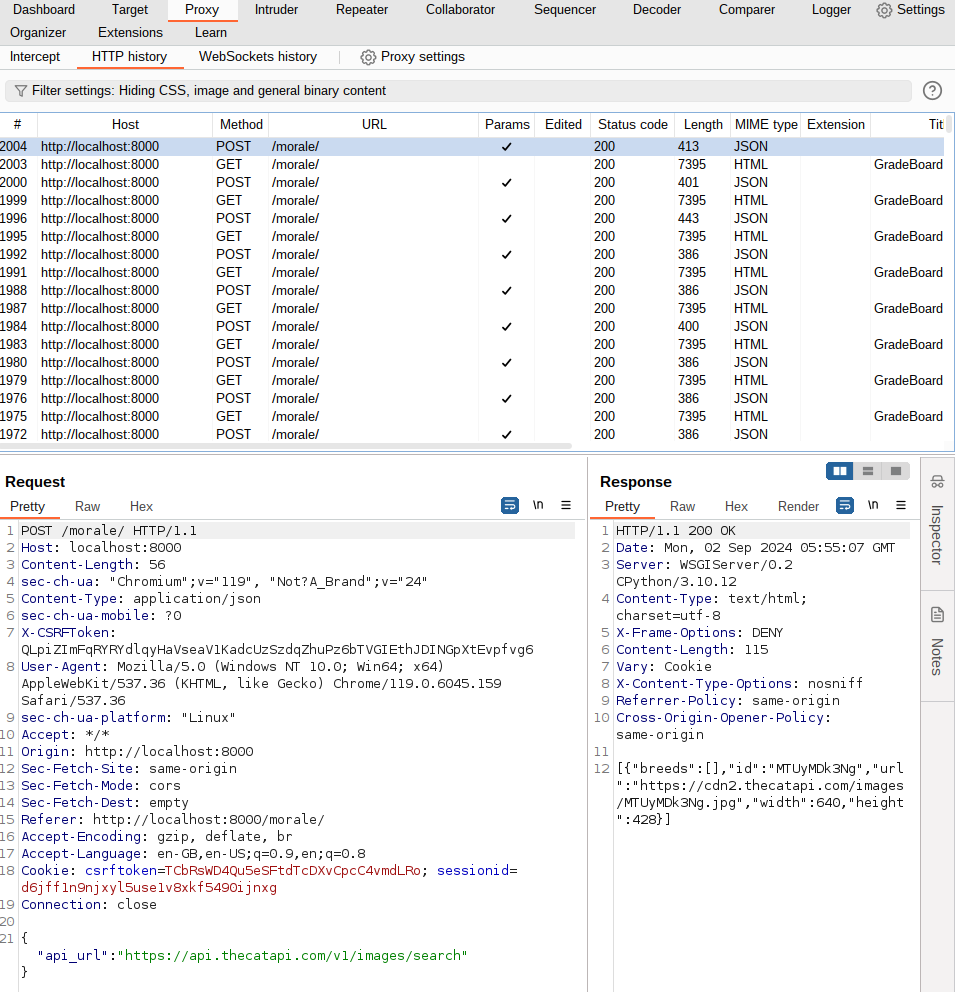
\includegraphics[width = \linewidth]{images/Michelle/catapifix.png}
\end{center}

Where appropriate POST requests can be intercepted with no API key leakage.

.env is already in .gitignore (for learning and execution purposes, .env will be included in the code repository, but normal practice would be to not include .env to prevent key leakage).

\begin{center}
    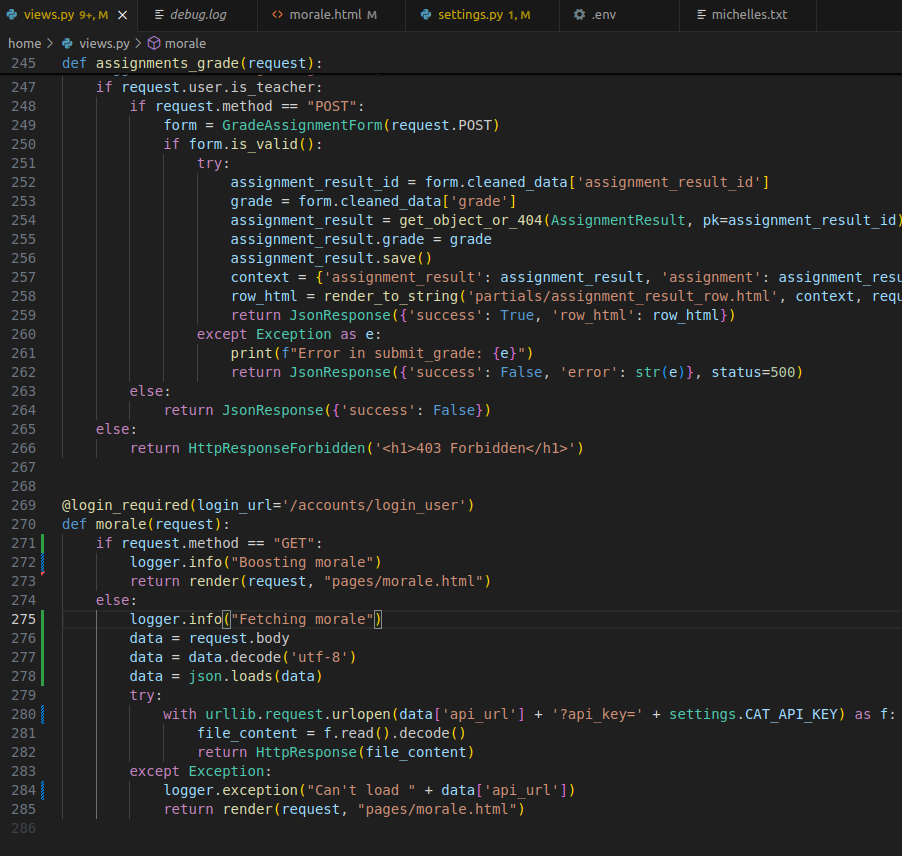
\includegraphics[width = \linewidth]{images/Michelle/viewschange.png}
\end{center}

\section{***Name of vulnerability***}

***Short written description of vulnerability***

\subparagraph{Investigation:}

***Describe how vulnerability was investigated. Use screenshots/suspicious network traces***

\subparagraph{Exploitation:}

*** discussion of the vulnerability found with the evidence gathered, i.e. you cannot simply jump into the code and/or database and point to the issue, but you must show how to exploit it and prove you did with screenshots and a walkthrough;***

\subparagraph{OWASP Top 10 Category:}

*** which category it belongs to using OWASP Top 10 2021 framework ***

\subparagraph{Corrective Action:}

*** what corrective action/s you applied in the code, explicitly referring to the location (file and line number) in the code, and briefly explaining the changes applied to the code including how this solves the vulnerability; ***